\begin{frame}
  \frametitle{V\&V Study 1: Verification of Moltres with the CNRS Benchmark}

  Published in \textit{S.M. Park, M. Munk, "Verification of Moltres for Multiphysics Simulations of
    Fast-Spectrum Molten Salt Reactors," Annals of Nuclear Energy, vol. 173, Aug 2022.}
  \begin{columns}
    \column[t]{6.5cm}
    \begin{block}{\textbf{CNRS Benchmark \cite{tiberga_results_2020}}}
      \begin{itemize}
        \item A numerical benchmark for multiphysics software dedicated to modeling ``pool-type''
          fast-spectrum MSRs
        \item Problem Setup
          \begin{itemize}
            \item LiF-BeF$_2$-UF$_4$ molten salt
            \item Six neutron energy groups
            \item Eight precursor groups
            \item Volumetric conjugate heat sink term
            \item Incompressible flow
          \end{itemize}
        \item Consists of three phases
          \begin{itemize}
            \item Phase 0: Single-physics verification
            \item Phase 1: Steady-state coupling
            \item Phase 2: Time-dependent coupling
          \end{itemize}
      \end{itemize}
    \end{block}
    \column[t]{3.5cm}
    \begin{figure}
      \centering
      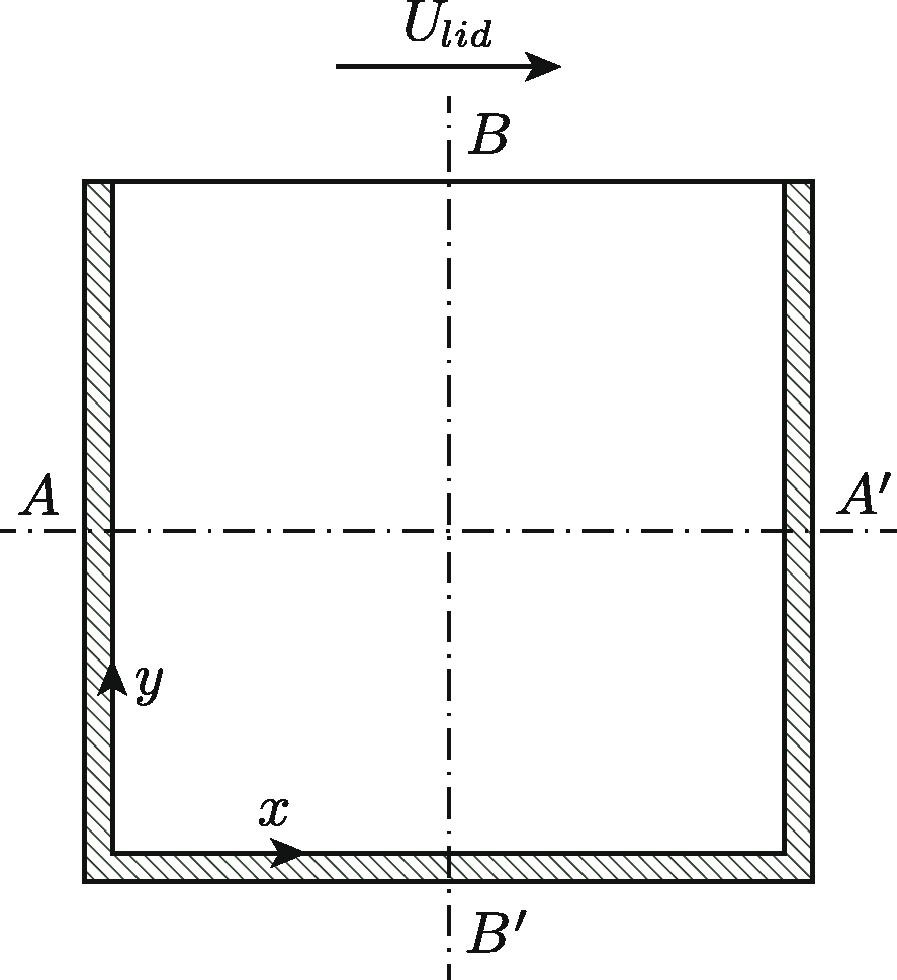
\includegraphics[width=\columnwidth]{../images/cnrs-geometry}
      \caption{CNRS benchmark problem domain \cite{tiberga_results_2020}}
    \end{figure}
  \end{columns}
\end{frame}

\begin{frame}
  \frametitle{V\&V Study 1: Verification of Moltres with the CNRS Benchmark}
  \textbf{Outcome: Moltres is consistent with the other multiphysics software in the benchmark
  problems.}
  \begin{columns}
    \hfill
    \column[t]{4cm}
    \vspace{.3cm}
    \begin{figure}
      \centering
      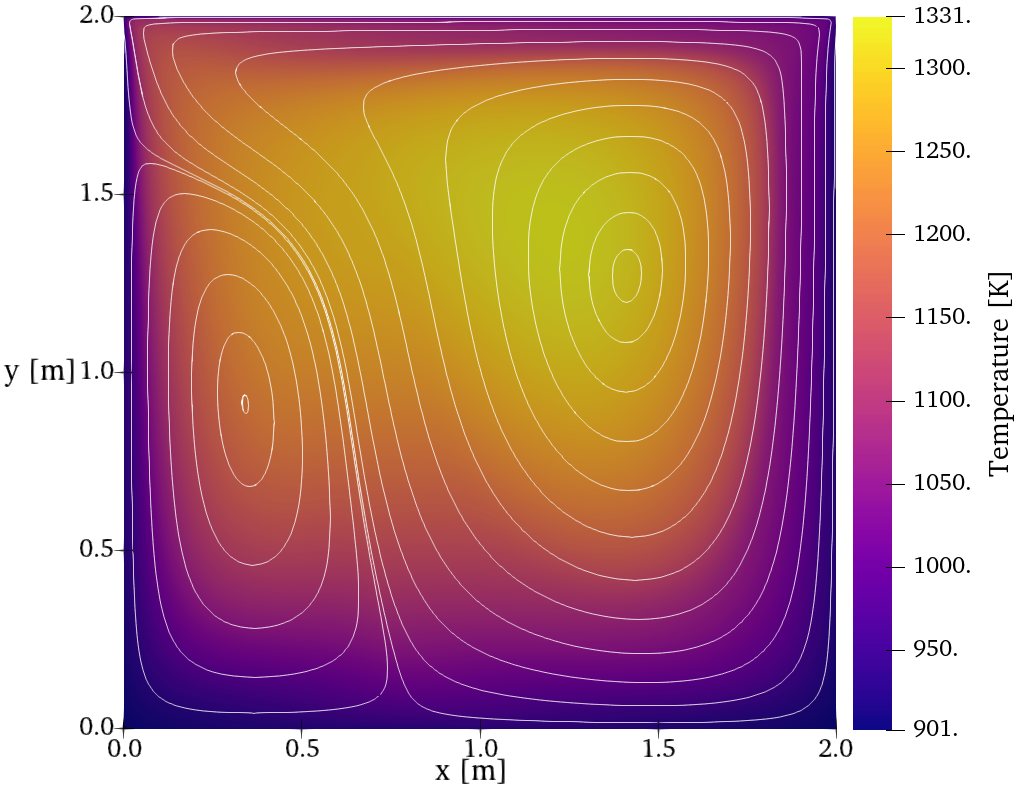
\includegraphics[width=\columnwidth]{../images/full-coupled}
      \caption{Step 1.4 - Temperature distribution and flow streamlines for the fully
      coupled system \cite{park_verification_2022}.}
    \end{figure}
    \column[t]{4cm}
    \begin{figure}
      \centering
      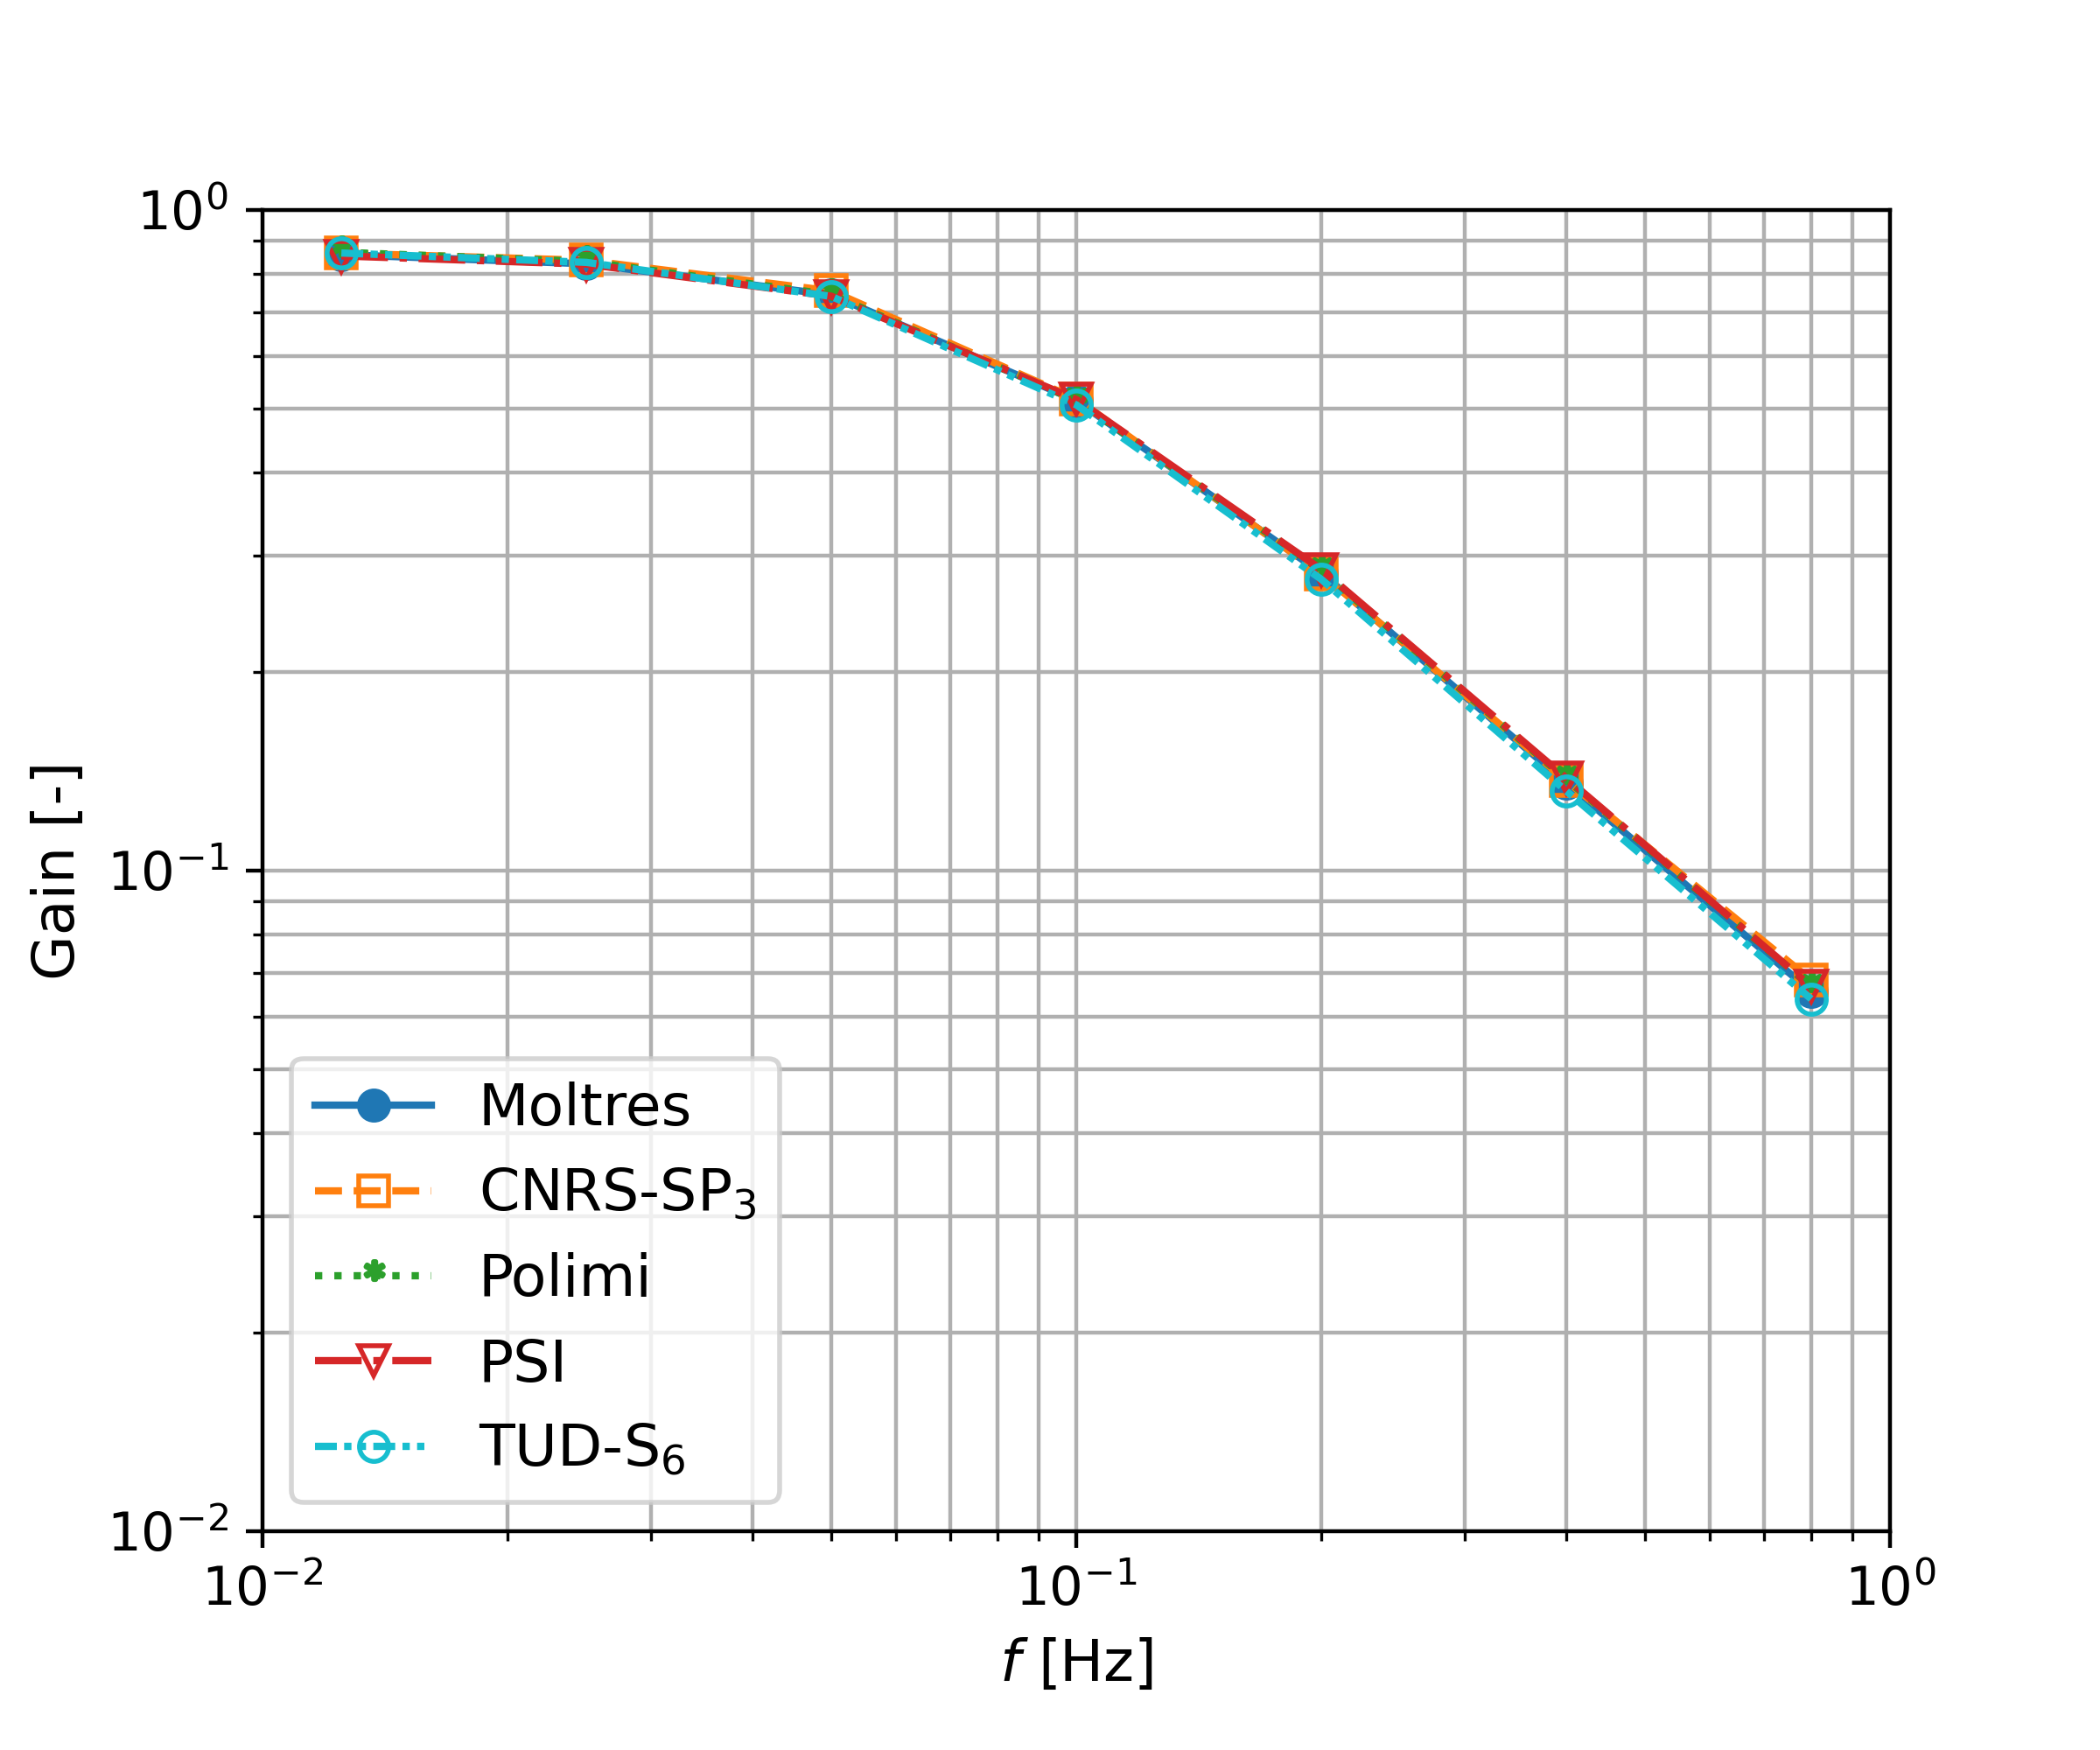
\includegraphics[width=\columnwidth]{../images/2-1-gain-plot}
      \caption{Step 2.1 - Bode gain plot of the frequency response of the fully
      coupled system \cite{park_verification_2022}.}
    \end{figure}
    \column[t]{4cm}
    \begin{figure}
      \centering
      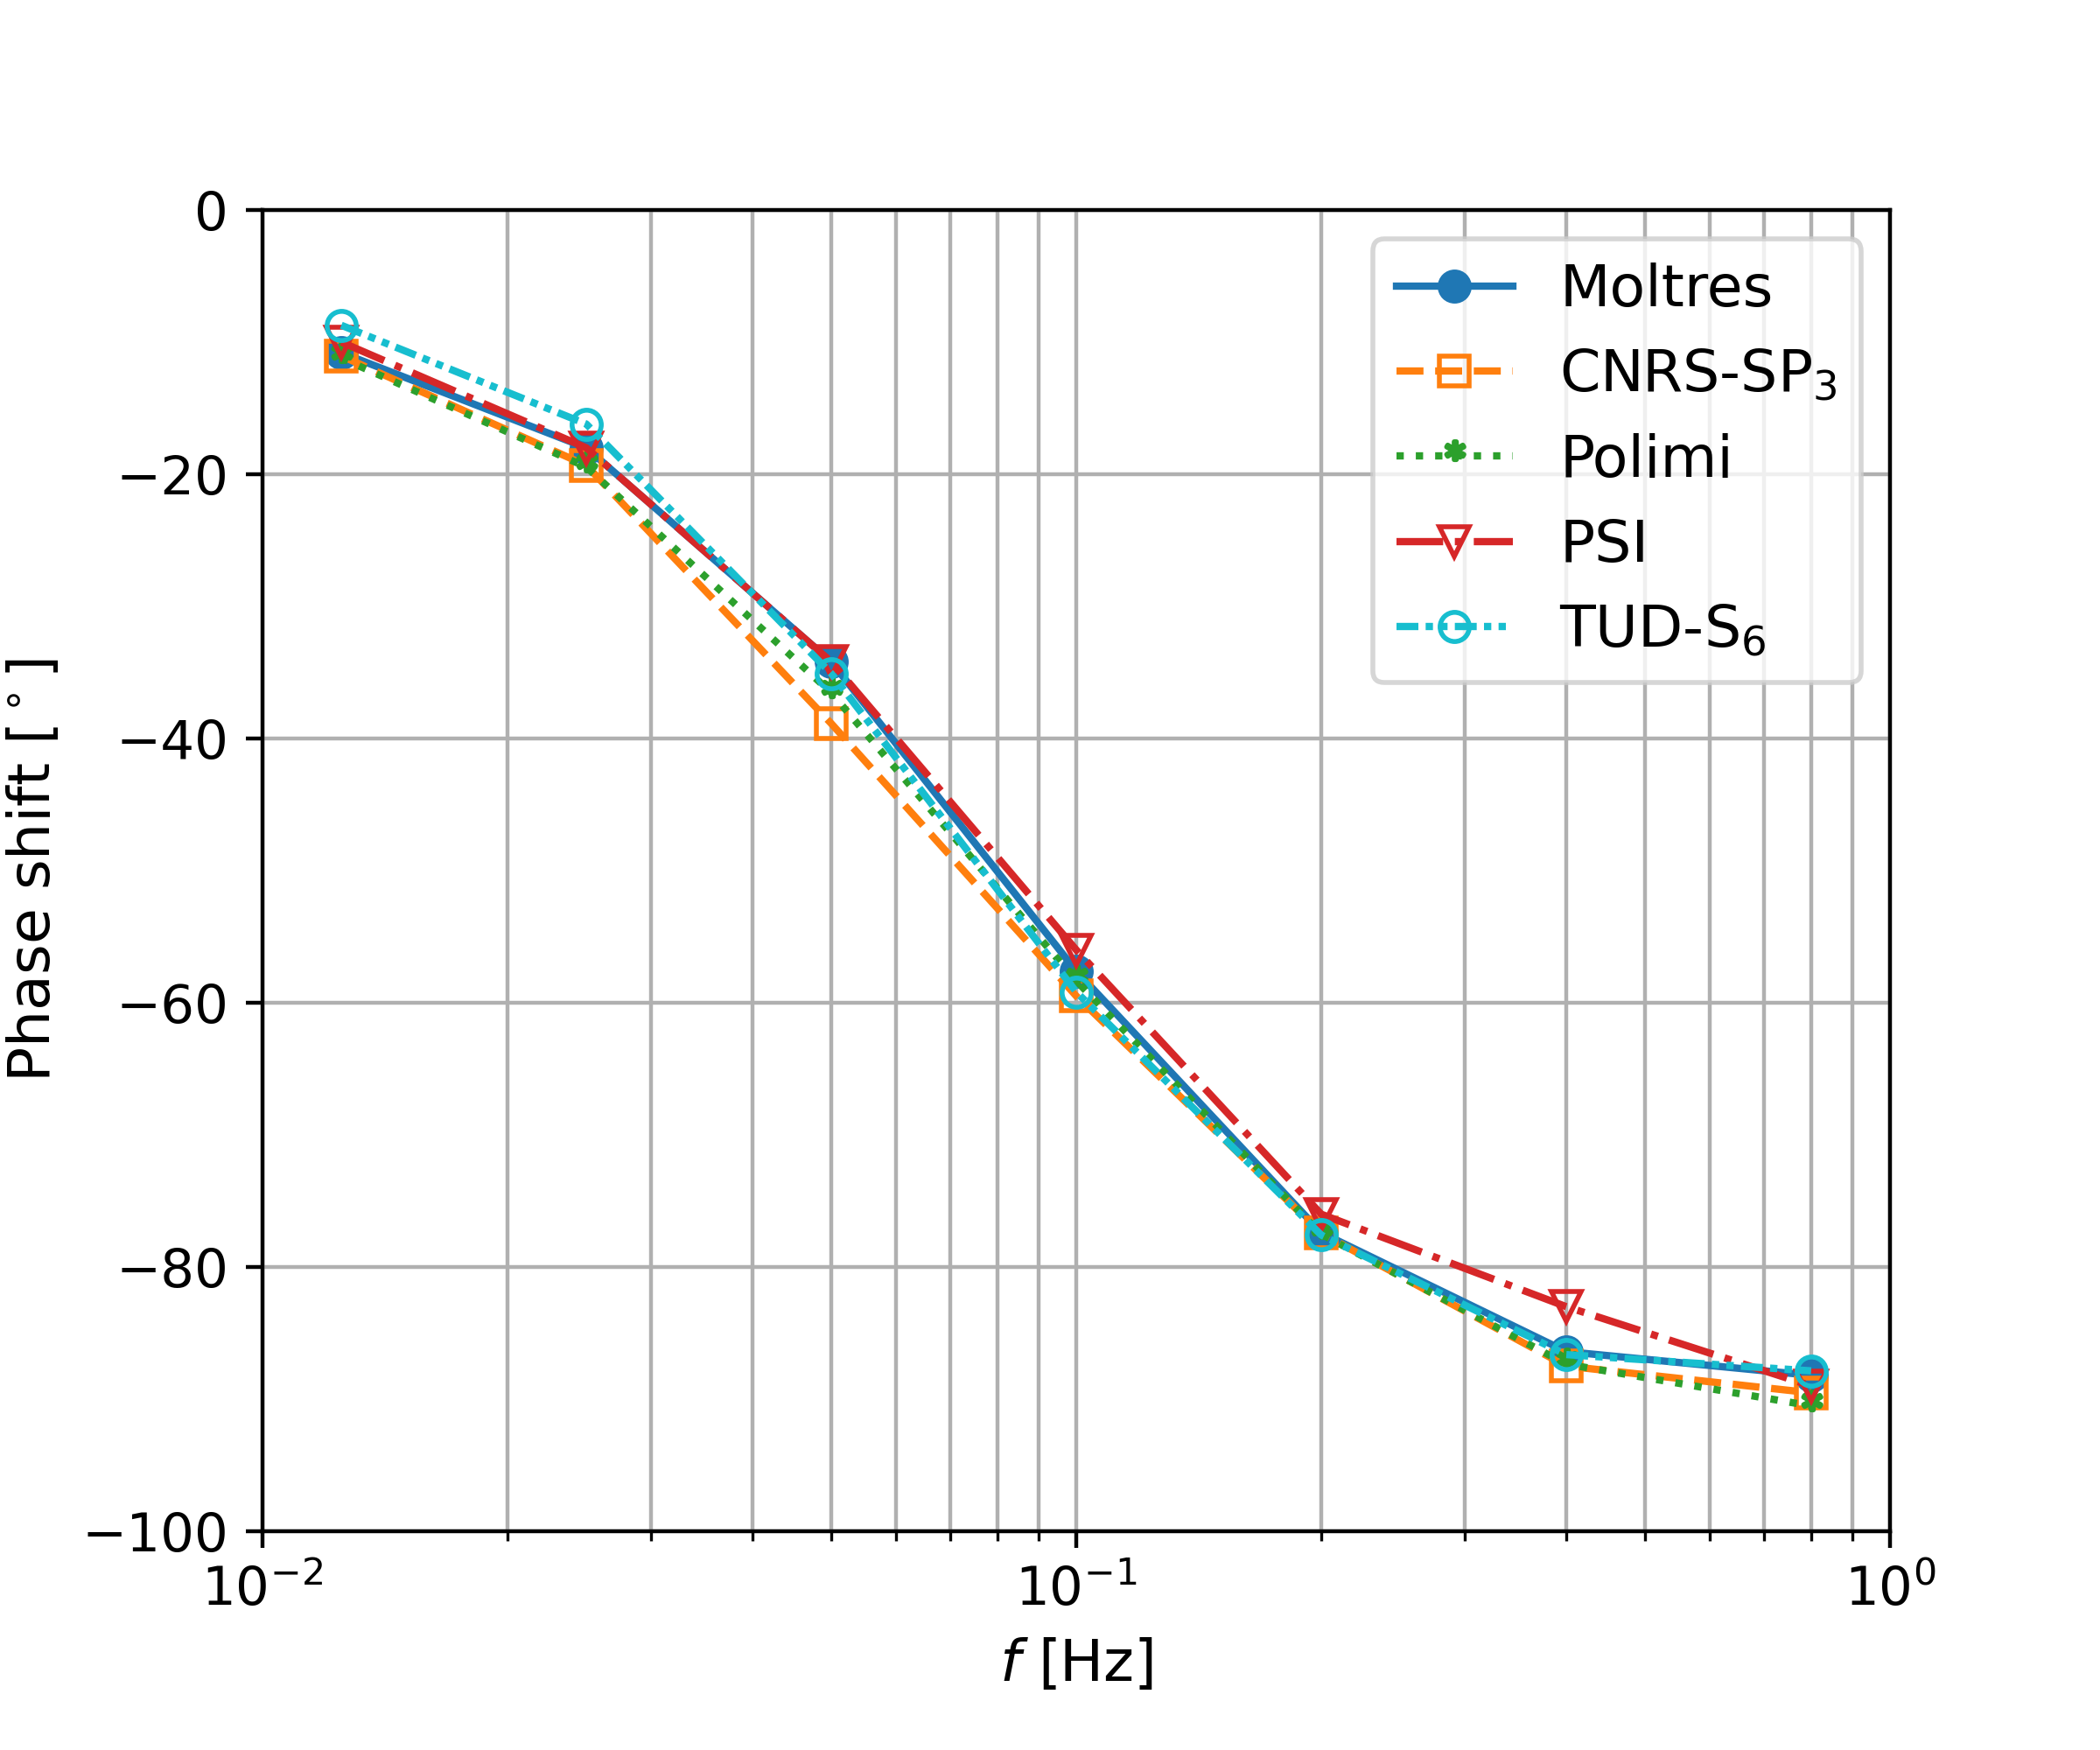
\includegraphics[width=\columnwidth]{../images/2-1-phase-plot}
      \caption{Step 2.1 - Bode phase plot of the frequency response of the fully
      coupled system \cite{park_verification_2022}.}
    \end{figure}
    \hfill
  \end{columns}
\end{frame}
